\documentclass[conference]{IEEEtran}

\usepackage[T1]{fontenc}
\usepackage{amsmath,amssymb}
\usepackage{graphicx}
\usepackage{subcaption}
\usepackage{booktabs}
\usepackage{xcolor}
\usepackage{cite}
\usepackage{url}
\DeclareMathOperator*{\argmin}{arg\,min}
\DeclareMathOperator*{\argmax}{arg\,max}

% Placeholder for content still to be written (renders in red; remove before submission)
\newcommand{\todo}[1]{\textcolor{red}{[TODO: #1]}}

% Include a figure if the file exists, otherwise draw a placeholder box
\newcommand{\safefig}[2][]{%
  \IfFileExists{../results/figures/#2}%
    {\includegraphics[width=#1\columnwidth]{../results/figures/#2}}%
    {\fbox{\parbox[c][3.5cm][c]{0.92\columnwidth}{\centering\small Missing figure:\\ \texttt{\detokenize{#2}}}}}%
}

\begin{document}

\title{ECSE 551 Assignment 1}

\author{\IEEEauthorblockN{Jocelyn Poon, Maxime Robatche-Claive, Louis Salanon, Ruiyong Xu}
\IEEEauthorblockA{Department of Electrical and Computer Engineering, McGill University, Montreal, Canada}}

\maketitle


% ==================================================================
\begin{abstract}
% 100-150 words. Grid: summarizes the work (1) and the findings (1).
% Name every model studied: ElasticNet, Lasso, LinearRegression, multiclass SVM, MLP, RandomForestClassifier,
% and for Task 3 the Lasso, random forest and MLP regressors.
A statistical analysis is first conducted on the Diabetes dataset for data processing, and then elastic net and lasso regression methods are implemented and compared to Scikit-learn's Linear Regression model. For the classification of the Digits dataset, One-vs-Rest Multiclass SVM and 2-layer MLP methods are implemented, and compared to Scikit-learn's Random Forest model. The custom Elastic Net model produced an MSE = 2773.64 and $R^2 = 0.4862$, the Lasso model produced an MSE = 2774.43 and $R^2 = 0.4861$, while the Scikit Learn Linear Regression model produced MSE = 2821.75 and $R^2 = 0.4773$, demonstrating similar results. The custom SVM and MLP models achieved 94.83\% and 96.66\% accuracies, respectively, while the Scikit-learn Random Forest model achieved 95.63\% accuracy, also demonstrating similar results. In Task 3, we predict the next-day volatility-adjusted returns of S\&P~500 stocks with a Lasso, a random forest and a multilayer perceptron trained in a walk-forward procedure, under a protocol designed to prevent lookahead and test-set overfitting. On the 2011--2013 test period, the random forest and the multilayer perceptron reach Sharpe ratios of 3.65 and 3.01, but most of this performance depends on trading at the closing prices used to form the predictions.
\end{abstract}


% ==================================================================
\section{Introduction}
% ==================================================================
% Grid: clearly presents the goals, all methods and all datasets (2). Introduce variables and acronyms.
The goal of this assignment is to perform exploratory data analysis and preprocessing (Task 1), implement and tune regression and classification models from scratch to compare against Scikit-learn baselines (Task 2), and predict next-day stock returns under a strict walk-forward evaluation protocol (Task 3). The Diabetes dataset contains information on 442 patients and 10 baseline variables, with the target variable as a continuous disease-progression target one year after baseline. We implement custom elastic net and lasso regression models with gradient descent and analyze the choice of parameters, and comparing them to Scikit-learn's Linear Regression model~\cite{sklearn}. For classification, we analyze the Digits dataset, which consists of 1797 $8\times 8$ grayscale images represented as 64 pixel features across 10 digit classes (0--9). We implement a One-vs-Rest multiclass support vector machine (SVM) and a two-layer multilayer perceptron (MLP) from scratch using gradient descent, comparing them to Scikit-learn's Random Forest Classifier~\cite{sklearn}. In Tasks 1 and 2, we find that feature scaling is essential for regularized gradient-based optimization, and that our custom Elastic Net, Lasso, SVM, and MLP models closely match or slightly outperform the Scikit-learn baselines when properly tuned. Task 3 uses daily returns of S\&P~500 constituents from 1980 to 2013 and social-media sentiment scores to predict which stocks will outperform the next day. We find genuine but small short-horizon predictability: nonlinear models outperform a linear model and simple trading rules on the test period, but their advantage largely disappears when trades are executed one day later.


% ==================================================================
\section{Task 1: Data Analysis and Preprocessing}
\label{sec:task1}
% ==================================================================

\subsection{Datasets}
% Grid: data cleaning and preprocessing steps clearly described (2).
\subsubsection{Diabetes}
The Diabetes dataset contains information about 442 patients and 10 real-valued baseline variables. The target variable measures disease progression one year after baseline. For preprocessing, it is determined that there are no missing features or values nor are there erroneous values to be cleaned. Comparing the original (Fig. ~\ref{fig:task1_regression_distributions_unscaled}) and scaled distributions (Fig. ~\ref{fig:task1_regression_distributions}) demonstrates that scaling centers the features around zero and makes their magnitudes more comparable. This is important for gradient based optimization and regularized regression, because features with different scales can negatively influence the regularization penalties. Fig. ~\ref{fig:task1_regression_boxplot} shows that outliers are present in most of the features, however, are not necessary to clean because medical variations exist and reflect diversities in human health.
\begin{figure}
    \centering
    \safefig{task1_regression_distributions_unscaled.png}
    \caption{Feature Distributions (Unscaled)}
    \label{fig:task1_regression_distributions_unscaled}
\end{figure}
\subsubsection{Digits}
The Digits data set consists of 1797 $8\times 8$ images of handwritten single digits labeled with the digits, so there are 64 features (one pixel each) and 10 labels (0--9). Each feature is an integer between 0 and 16 (inclusive) that indicates the grayscale intensity of a pixel. The data set is linted to check for any missing or out-of-range feature values or label values, and none are found. As shown by Fig.~\ref{fig:digits_pixel_intensity_distribution}, the pixel intensity spreads across the entire range and concentrates at the minimum and the maximum. The distribution of the total amount of ink in a digit image, as defined by the sum of pixel intensities, is shown in Fig.~\ref{fig:digits_ink_amount_distribution}. It approximates a bell curve and there is no notable abnormality.

\begin{figure}[t]
\centering
\safefig[0.8]{digits_pixel_intensity_distribution.png}
\caption{Pixel intensity distribution in digits}
\label{fig:digits_pixel_intensity_distribution}
\end{figure}

\begin{figure}[t]
\centering
\safefig[0.9]{digits_ink_amount_distribution.png}
\caption{Distribution of the total amount of ink in a digit image}
\label{fig:digits_ink_amount_distribution}
\end{figure}

\subsection{Statistical Analysis}
% Grid: statistical data analysis included, e.g. means, box plots, correlations (1).
% Assignment questions: means, min/max, need for scaling, modality, heavy tails vs Gaussian, discrete features, correlated features.
\subsubsection{Diabetes}
Fig.~\ref{fig:task1_regression_distributions} shows the histograms of all the features, showing that several features have approximately bell shaped distributions centered around one mode, although some exhibit skewness. Fig.~\ref{fig:task1_regression_boxplot} are the box plots showing the distribution and variability of each feature. Sex is represented by two numerical categories, but as it is a categorical variable, its box plot is not very informative. Finally, Fig.~\ref{fig:task1_regression_corr_matrix} shows the correlation coefficients between features and the target while Fig.~\ref{fig:task1_regression_correlations} shows scatter plots of moderately positive correlations. Strong correlations between features show multicollinearity, where multiple features have overlapping information.
\begin{table}[htbp]
\centering
\caption{Statistics of the Diabetes Dataset}
\label{tab:diabetes_stats}
\resizebox{0.48\textwidth}{!}{%
\begin{tabular}{lrrrrrrrrrr}
\hline
 & age & sex & bmi & bp & s1 & s2 & s3 & s4 & s5 & s6 \\
\hline
count & 442.000 & 442.000 & 442.000 & 442.000 & 442.000 & 442.000 & 442.000 & 442.000 & 442.000 & 442.000 \\
mean  & 48.518 & 1.468 & 26.376 & 94.647 & 189.140 & 115.439 & 49.788 & 4.070 & 4.641 & 91.260 \\
std   & 13.109 & 0.500 & 4.418 & 13.831 & 34.608 & 30.413 & 12.934 & 1.290 & 0.522 & 11.496 \\
min   & 19.000 & 1.000 & 18.000 & 62.000 & 97.000 & 41.600 & 22.000 & 2.000 & 3.258 & 58.000 \\
25\%  & 38.250 & 1.000 & 23.200 & 84.000 & 164.250 & 96.050 & 40.250 & 3.000 & 4.277 & 83.250 \\
50\%  & 50.000 & 1.000 & 25.700 & 93.000 & 186.000 & 113.000 & 48.000 & 4.000 & 4.621 & 91.000 \\
75\%  & 59.000 & 2.000 & 29.275 & 105.000 & 209.750 & 134.500 & 57.750 & 5.000 & 4.997 & 98.000 \\
max   & 79.000 & 2.000 & 42.200 & 133.000 & 301.000 & 242.400 & 99.000 & 9.090 & 6.107 & 124.000 \\
\hline
\end{tabular}%
}
\end{table}
\begin{figure}
    \centering
    \safefig{task1_regression_distributions.png}
    \caption{Feature Distributions (Scaled)}
    \label{fig:task1_regression_distributions}
\end{figure}
\begin{figure}
    \centering
    \safefig{task1_regression_corr_matrix.png}
    \caption{Feature Correlation}
    \label{fig:task1_regression_corr_matrix}
\end{figure}
\begin{figure}
    \centering
    \safefig{task1_regression_correlations.png}
    \caption{Examples of Correlated Features}
    \label{fig:task1_regression_correlations}
\end{figure}
\begin{figure}
    \centering
    \safefig{task1_regression_boxplot.png}
    \caption{Box Plots of Features}
    \label{fig:task1_regression_boxplot}
\end{figure}

\subsubsection{Digits}

Fig.~\ref{fig:digits_class_sizes} shows the sample sizes of different digits, demonstrating that the class sizes are balanced. The mean digit image is shown in Fig.~\ref{fig:digits_mean_image}. Pixels are generally dimmer near the left and right edges, but the middle of the top and the bottom edges have the strongest mean pixel intensities. Fig.~\ref{fig:digits_image_variance} shows the heat map of pixel intensity variance, indicating that the variance is the highest near the center. The pixels on the left and right edges have a zero or near zero variance, indicating that all or most of those pixels have a constant value, which, based on the mean image, is zero. 

\begin{figure}[t]
\centering
\safefig[0.9]{digits_class_sizes.png}
\caption{Class sizes of the Digits dataset}
\label{fig:digits_class_sizes}
\end{figure}

\begin{figure}[t]
\centering
\begin{subfigure}[t]{0.45\columnwidth}
\safefig{digits_mean_image.png}
\caption{Mean image}
\label{fig:digits_mean_image}
\end{subfigure}
\begin{subfigure}[t]{0.45\columnwidth}
\safefig{digits_image_variance.png}
\caption{Variance of image}
\label{fig:digits_image_variance}
\end{subfigure}
\caption{Heatmaps of the pixel intensity mean and variance of digits}
\end{figure}


% ==================================================================
\section{Task 2: Models Implemented from Scratch}
\label{sec:task2}
% ==================================================================

\subsection{Methodology}
% Grid (Methodology): ElasticNet with loss (2), Lasso with soft thresholding and loss (2), LinearRegression (2),
% MLP with loss (2), SVM with hinge loss and one-vs-rest (2), RandomForestClassifier (2),
% metrics MSE and accuracy mentioned (0.5) and explained (1), description of model training (1).
% Also: define hyperparameters, state the 70/30 split with random state 42, and how hyperparameters were tuned.

\textit{Evaluation.} The hyperparameters of the Elastic Net and Lasso models were tuned using a one at a time, where each hyperparameter was varied independently while the remaining parameters were held constant at their baseline values. For both the regression task and the classification task, the data sets are split using a train/test split of 70\% / 30\% and a random state of 42. MSE measures the average of the squared differences between predicted values and true values, given as:

\begin{equation}
    \mathrm{MSE} = \frac{1}{n}\sum_{i=1}^{n}(y_i-\hat{y}_i)^2
\end{equation}
For the diabetes dataset, $R^2$ is appropriate for accuracy measurement:

\begin{equation}
    R^2 = 1 -
    \frac{\sum_{i=1}^{n}(y_i-\hat{y}_i)^2}
    {\sum_{i=1}^{n}(y_i-\bar{y})^2}
\end{equation}


\subsubsection{ElasticNet Regression}
For weights $\mathbf w$, bias $b$ and $N$ training pairs $(\mathbf x_j, y_j)$, ElasticNet minimizes
\begin{equation}
\mathcal L(\mathbf w, b) = \frac{1}{2N}\sum_{j=1}^{N}\bigl(y_j - \mathbf w^\top\mathbf x_j - b\bigr)^2 + \lambda_1\lVert\mathbf w\rVert_1 + \frac{\lambda_2}{2}\lVert\mathbf w\rVert_2^2.
\end{equation}
For gradient descent, the weight and bias updates are as follows:
\begin{equation}
\small
\mathbf{W}^{(t+1)} = \mathbf{W}^{(t)} - \eta \left[
\frac{1}{N}\mathbf{X}^T(\hat{\mathbf{Y}}-\mathbf{Y})
+ \lambda_1 \operatorname{sign}(\mathbf{W}^{(t)})
+\lambda_2\mathbf{W}^{(t)}
\right]
\end{equation}

\begin{equation}
b^{(t+1)} = b^{(t)} - \eta \frac{1}{N}
\sum_{i=1}^{N}(\hat{y}_i-y_i)
\end{equation}
where $\lambda_1$ controls the strength of the $L_1$ penalty (sparsity and feature selection) and $\lambda_2$ controls the strength of the $L_2$ penalty (shrinking and correlated weights together).

\subsubsection{Lasso Regression with Soft Thresholding}
The Lasso is the special case $\lambda_2 = 0$. Lasso minimizes
\begin{equation}
\mathcal{L}(W, b) = \frac{1}{2m} \sum_{i=1}^{m} \left( \hat{y}^{(i)} - y^{(i)} \right)^2 + \lambda_1 \sum_{j=1}^{n} |w_j|
\end{equation}
For gradient descent, the weight and bias updates are as follows:
\begin{equation}
\nabla_W \mathcal{L}_{\text{OLS}} = \frac{1}{m} X^T (\hat{Y} - Y)
\end{equation}
\begin{equation}
\nabla_b \mathcal{L}_{\text{OLS}} = \frac{1}{m} \sum_{i=1}^{m} (\hat{y}^{(i)} - y^{(i)})
\end{equation}
From soft thresholding
\begin{equation}
W_{\text{temp}} = W - \eta \cdot \nabla_W \mathcal{L}_{\text{OLS}}
\end{equation}
\begin{equation}
W^{(t+1)} = \mathcal{S}\left(W_{\text{temp}}, \eta \lambda_1\right)
\end{equation}
\begin{equation}
\mathcal{S}(x, \gamma) = \text{sign}(x) \cdot \max(|x| - \gamma, 0)
\end{equation}
with $\gamma = \eta \cdot \lambda_1$ which is the threshold value.
\begin{equation}
b^{(t+1)} = b^{(t)} - \eta \nabla_b\mathcal{L}_{OLS}
\end{equation}
\subsubsection{Linear Regression}
Scikit-learn's Linear Regression uses ordinary least squares:
\begin{equation}
\mathcal{L}(W,b) = \frac{1}{2m}
\sum_{i=1}^{m}
\left(\hat{y}^{(i)} - y^{(i)}\right)^2
\end{equation}

\begin{equation}
\nabla_W \mathcal{L} =
\frac{1}{m}X^T(\hat{Y}-Y)
\end{equation}

\begin{equation}
\nabla_b \mathcal{L} =
\frac{1}{m}\sum_{i=1}^{m}
\left(\hat{y}^{(i)}-y^{(i)}\right)
\end{equation}


\begin{equation}
W^{(t+1)} = W^{(t)} - \eta \nabla_W \mathcal{L}
\end{equation}

\begin{equation}
b^{(t+1)} = b^{(t)} - \eta \nabla_b \mathcal{L}
\end{equation}



\subsubsection{Multiclass SVM}
For a binary problem with labels $t_j \in \{-1, +1\}$, a linear SVM predicts with $f(\mathbf x) = \mathbf w^\top\mathbf x + b$, where $\mathbf w$ are the weights and $b$ is the bias. It is trained by minimizing the L2-regularized hinge loss
\begin{equation}
\mathcal L = \frac{\lambda}{2}\lVert\mathbf w\rVert_2^2 + \frac{1}{N}\sum_{j=1}^{N}\max\bigl(0,\, 1 - t_j f(\mathbf x_j)\bigr),
\label{eq:hinge}
\end{equation}
where $\lambda$ is the regularization parameter. The hinge loss is not differentiable where $t_j f(\mathbf x_j) = 1$, and we take its subgradient to be zero there. With $\mathcal S = \{j : t_j f(\mathbf x_j) < 1\}$, the set of samples that are misclassified or inside the margin, the subgradients of~\eqref{eq:hinge} are
\begin{equation}
\nabla_{\mathbf w}\mathcal L = \lambda\mathbf w - \frac{1}{N}\sum_{j\in\mathcal S} t_j\mathbf x_j, \qquad
\frac{\partial\mathcal L}{\partial b} = -\frac{1}{N}\sum_{j\in\mathcal S} t_j .
\end{equation}
Starting from $\mathbf w = \mathbf 0$ and $b = 0$, subgradient descent with learning rate $\eta$ repeats $\mathbf w \leftarrow \mathbf w - \eta\nabla_{\mathbf w}\mathcal L$ and $b \leftarrow b - \eta\,\partial\mathcal L/\partial b$ for a fixed number of iterations, using all training samples at each step. For the ten digit classes, we use one-vs-rest (OvR): for each class $k \in \{0, \ldots, 9\}$, a binary SVM $f_k$ is trained with $t_j = 1$ if $y_j = k$ and $t_j = -1$ otherwise, and a sample is assigned to the class with the highest score, $\hat y = \argmax_k f_k(\mathbf x)$. The hyperparameters are $\lambda$, $\eta$ and the number of iterations.

\subsubsection{Multilayer Perceptron}
The MLP has $n_0 = 64$ input units, one hidden layer of $n_1$ units with the rectified linear unit (ReLU) activation, $\mathrm{ReLU}(z) = \max(0, z)$, and $n_2 = 10$ softmax output units. Its parameters are the weight matrices $W^{(1)} \in \mathbb R^{n_1\times n_0}$ and $W^{(2)} \in \mathbb R^{n_2\times n_1}$ and the bias vectors $\mathbf b^{(1)} \in \mathbb R^{n_1}$ and $\mathbf b^{(2)} \in \mathbb R^{n_2}$. For an input $\mathbf x$, the forward pass computes
\begin{gather}
\mathbf z^{(1)} = W^{(1)}\mathbf x + \mathbf b^{(1)}, \qquad \mathbf a^{(1)} = \mathrm{ReLU}\bigl(\mathbf z^{(1)}\bigr), \nonumber\\
f(\mathbf x) = \sigma\bigl(W^{(2)}\mathbf a^{(1)} + \mathbf b^{(2)}\bigr),
\end{gather}
where ReLU is applied elementwise and $\sigma$ is the softmax, $\sigma(\mathbf z)_c = e^{z_c}/\sum_{k} e^{z_k}$, so that $f(\mathbf x)_c$ is the predicted probability of class $c$. With $\tilde{\mathbf y}_j$ the one-hot encoding of the class $y_j$ of sample $\mathbf x_j$, the model minimizes the cross-entropy loss
\begin{equation}
\mathcal L = -\frac{1}{N}\sum_{j=1}^{N}\sum_{c=1}^{n_2}(\tilde{\mathbf y}_j)_c\log f(\mathbf x_j)_c = -\frac{1}{N}\sum_{j=1}^{N}\log f(\mathbf x_j)_{y_j}.
\end{equation}
For softmax with cross-entropy, the gradient with respect to the output pre-activation of sample $j$ simplifies to $\boldsymbol\delta^{(2)}_j = f(\mathbf x_j) - \tilde{\mathbf y}_j$. Backpropagation then gives
\begin{gather*}
\nabla_{W^{(2)}}\mathcal L = \frac{1}{N}\sum_{j=1}^{N}\boldsymbol\delta^{(2)}_j\,\mathbf a^{(1)\top}_j, \qquad
\nabla_{\mathbf b^{(2)}}\mathcal L = \frac{1}{N}\sum_{j=1}^{N}\boldsymbol\delta^{(2)}_j,\\
\boldsymbol\delta^{(1)}_j = \bigl(W^{(2)\top}\boldsymbol\delta^{(2)}_j\bigr)\odot\mathrm{ReLU}'\bigl(\mathbf z^{(1)}_j\bigr),\\
\nabla_{W^{(1)}}\mathcal L = \frac{1}{N}\sum_{j=1}^{N}\boldsymbol\delta^{(1)}_j\,\mathbf x_j^\top, \qquad
\nabla_{\mathbf b^{(1)}}\mathcal L = \frac{1}{N}\sum_{j=1}^{N}\boldsymbol\delta^{(1)}_j,
\end{gather*}
where $\odot$ is the elementwise product and $\mathrm{ReLU}'(z) = 1$ if $z > 0$ and $0$ otherwise. Weights are initialized from a normal distribution with standard deviation 0.001 (random seed 42) to break the symmetry between hidden units, and biases at zero. Each epoch performs one full-batch gradient-descent step $\theta \leftarrow \theta - \eta\nabla_\theta\mathcal L$ on every parameter $\theta$, with learning rate $\eta$. The hyperparameters are the hidden size $n_1$, $\eta$ and the number of epochs.

\subsubsection{Random Forest}
A random forest is an ensemble of decision trees that produces a decision based on majority voting. For each tree, a bootstrap sample is created by bagging, i.e., drawing training samples with replacement. The decision tree is grown by splitting nodes. At each split, only a random subset of the available features is considered. At each node, the tree chooses the split that minimizes the Gini impurity $G$, as defined by
\[
G = 1 - \sum_{k=1}^{K}p_k^2
\]
where $p_k$ is the proportion of class $k$ in the node. A candidate split is evaluated using its weighted child impurity, defined by
\[
G_{\text{split}} = \frac{n_L}{n}G_L + \frac{n_R}{n}G_R
\]
where $n_L$ and $n_R$ are the sample counts of the left and right children, respectively, and $G_L$ and $G_R$ are their Gini impurity. The tree recursively chooses the split that minimizes $G_{\text{split}}$, until a leaf node or the maximum depth is reached.

For prediction, given a new input $x$, every tree produces a class prediction. The forest returns the majority vote, that is, the class that's predicted by the most trees.

\subsection{Results}
% Grid (Results): ElasticNet/Lasso results interpreted correctly (2), SVM decision boundaries and performance (1),
% MLP architecture and hyperparameter analysis (1), comparison between scratch and scikit-learn models (2),
% results presented with clear figures/tables (2).
% Always state the range of each hyperparameter tested and the best values.

\subsubsection{Elastic Net.} 
\begin{figure}
    \centering
    \safefig{task2_elasticnet_pvsa.png}
    \caption{Elastic Net Predicted vs. Actual}
    \label{fig:task2_elasticnet_pvsa.png}
\end{figure}
\begin{figure}
    \centering
    \safefig{task2_elasticnet_residual.png}
    \caption{Elastic Net Residual}
    \label{fig:task2_elasticnet_residual.png}
\end{figure}
\begin{figure}
    \centering
    \safefig{task2_elasticnet_featurecomp.png}
    \caption{Elastic Net Feature Comparison}
    \label{fig:task2_elasticnet_featurecomp.png}
\end{figure}
\begin{figure}
    \centering
    \safefig{task2_elasticnet_lr.png}
    \caption{Elastic Net Learning Rate}
    \label{fig:task2_elasticnet_lr.png}
\end{figure}
\begin{figure}
    \centering
    \safefig{task2_elasticnet_l1.png}
    \caption{Elastic Net $L_1$ Ratio}
    \label{fig:task2_elasticnet_l1.png}
\end{figure}
\begin{figure}
    \centering
    \safefig{task2_elasticnet_alpha.png}
    \caption{Elastic Net Alpha}
    \label{fig:task2_elasticnet_alpha.png}
\end{figure}
\begin{figure}
    \centering
    \safefig{task2_elasticnet_iterperform.png}
    \caption{Elastic Net Iterations}
    \label{fig:task2_elasticnet_iterperform.png}
\end{figure}
\begin{figure}
    \centering
    \safefig{task2_elasticnet_l2.png}
    \caption{Elastic Net $L_2$ Ratio}
    \label{fig:task2_elasticnet_l2.png}
\end{figure}
The custom Elastic Net model produced an MSE= 2773.64 and $R^2 = 0.4862$ while the Scikit Learn Linear Regression model produced MSE = 2821.75 and $R^2 = 0.4773$, demonstrating similar results. Fig.~\ref{fig:task2_elasticnet_pvsa.png} shows the predictions of the custom model and Scikit-learn's Linear Regression model against the true diabetes progression values. Both models produce predictions that generally follow the positive relationship between actual and predicted disease progression.
Fig.~\ref{fig:task2_elasticnet_featurecomp.png} illustrates the differences between the coefficients learned by both models. The $L_1$ and $L_2$ penalties were able to push certain coefficients toward zero and induce sparsity, reducing the influence of redundant or less useful features. Some coefficients remain relatively similar between the two models, indicating that those features are important in prediction. The $L_1$ and $L_2$ ratios are defined in the custom model as $\alpha \cdot L$ratio.
Fig.~\ref{fig:task2_elasticnet_l1.png}, Fig.~\ref{fig:task2_elasticnet_l2.png}, Fig.~\ref{fig:task2_elasticnet_alpha.png}, and Fig.~\ref{fig:task2_elasticnet_iterperform.png} show how the choice of parameters affects the model's performance.

\begin{table}[htbp]
    \centering
    \caption{Elastic Net Hyperparameter Optimization Results}
    \label{tab:elasticnet_hyperparameters}
    \begin{tabular}{|l|c|c|}
        \hline
        \textbf{Hyperparameter} & \textbf{Tested Range} & \textbf{Best Value} \\
        \hline
        Learning Rate & 0.001--0.2 & 0.025 \\
        \hline
        Iterations & 100--10,000 & 500 \\
        \hline
        Alpha ($\alpha$) & 0.001--1.0 & 0.05 \\
        \hline
        L1 Ratio & 0--1 & 0.5 \\
        \hline
        L2 Ratio & 0--1 & 0.5 \\
        \hline
    \end{tabular}
\end{table}

\subsubsection{Lasso.}
\begin{figure}
    \centering
    \safefig{task2_lasso_pvsa.png}
    \caption{Lasso Predicted vs. Actual}
    \label{fig:task2_lasso_pvsa.png}
\end{figure}
\begin{figure}
    \centering
    \safefig{task2_lasso_residual.png}
    \caption{Lasso Residual}
    \label{fig:task2_lasso_residual.png}
\end{figure}
\begin{figure}
    \centering
    \safefig{task2_lasso_featurecomp.png}
    \caption{Lasso Feature Comparison}
    \label{fig:task2_lasso_featurecomp.png}
\end{figure}
\begin{figure}
    \centering
    \safefig{task2_lasso_lr.png}
    \caption{Lasso Learning Rate}
    \label{fig:task2_lasso_lr.png}
\end{figure}
\begin{figure}
    \centering
    \safefig{task2_lasso_l1.png}
    \caption{Lasso $L_1$ Ratio}
    \label{fig:task2_lasso_l1.png}
\end{figure}
\begin{figure}
    \centering
    \safefig{task2_lasso_alpha.png}
    \caption{Lasso Alpha}
    \label{fig:task2_lasso_alpha.png}
\end{figure}
\begin{figure}
    \centering
    \safefig{task2_lasso_iterperform.png}
    \caption{Lasso Iterations}
    \label{fig:task2_lasso_iterperform.png}
\end{figure}
The custom Lasso model produced an MSE= 2774.43 and $R^2 = 0.4861$ while the Scikit Learn Linear Regression model produced MSE = 2821.75 and $R^2 = 0.4773$. Fig.~\ref{fig:task2_lasso_pvsa.png} examines the predictions of the custom model and Scikit-learn's Linear Regression model against the true diabetes progression values. Like the elastic net analysis, both models produce predictions that generally follow the positive relationship between actual and predicted disease progression.
Fig.~\ref{fig:task2_lasso_featurecomp.png} illustrates the differences between the coefficients learned by both models. The $L_1$ penalty was able to push certain coefficients toward zero, reducing the influence of redundant or less useful features. Again, some coefficients remain relatively similar between the two models, indicating that those features are important in prediction.
Fig.~\ref{fig:task2_lasso_l1.png}, Fig.~\ref{fig:task2_lasso_alpha.png}, and Fig.~\ref{fig:task2_lasso_iterperform.png} show how the choice of parameters affects the model's performance.
\begin{table}[htbp]
    \centering
    \caption{Lasso Hyperparameter Optimization Results}
    \label{tab:elasticnet_hyperparameters}
    \begin{tabular}{|l|c|c|}
        \hline
        \textbf{Hyperparameter} & \textbf{Tested Range} & \textbf{Best Value} \\
        \hline
        Learning Rate & 0.001--0.2 & 0.025 \\
        \hline
        Iterations & 100--10,000 & 500 \\
        \hline
        Alpha ($\alpha$) & 0.001--1.0 & 0.1 \\
        \hline
        L1 Ratio & 0--1 & 0.75 \\
        \hline
    \end{tabular}
\end{table}

\subsubsection{Multiclass SVM}
For tunning the SVM model, a grid search is performed for regularization parameter $\lambda$ and learning rate $\eta$, with the number of iterations set to a fixed value. The ranges of $\lambda$ and $\eta$ are shown in the $x$-axis of Fig.~\ref{fig:digits_svm_accuracy_vs_lambda} and Fig.~\ref{fig:digits_svm_accuracy_vs_lr}. At each point in the grid, the performance is evaluated as the mean accuracy in a 5-fold cross-validation. This procedure is repeated for different numbers of iterations $n_{\text{iter}}$ until $n_{\text{iter}}$ is just large enough that the best performance plateaus. The gray vertical lines in Fig.~\ref{fig:digits_svm_accuracy_vs_lambda} and Fig.~\ref{fig:digits_svm_accuracy_vs_lr} indicate the best hyperparameter values. The chosen values are
\[
\lambda = 10^{-4},\qquad\eta = 0.01,\qquad n_{\text{iter}} = 400
\]
With these hyperparameters, the accuracy on the test set is $94.83\%$.

Increasing $\lambda$ results in underfitting while decreasing it results in overfitting, both degrading accuracy on unseen data, as Fig.~\ref{fig:digits_svm_accuracy_vs_lambda} shows. If the learning rate is large, the gradient descent will overshoot, and if it is small then the point of convergence cannot be reached in a fixed number of iterations, both reducing the performance, as Fig.~\ref{fig:digits_svm_accuracy_vs_lr} shows.

Since the data has 64 features, in order to plot the decision boundary, the dimension must be reduced. We do it by using PCA to project the data points to 2-D. We then train a SVM model on the 2-D data set, using grid search to tune the hyperparameters. The result is plotted in Fig.~\ref{fig:digits_svm_decision_boundaries}. Each scattered point is a sample while the regions of different colors are decision regions. The cross-validation accuracy on this data set is only $56.43\%$, apparently due to the loss of important information about features in the projection.
\begin{figure}[t]
\centering
\safefig[0.75]{digits_svm_accuracy_vs_lambda.png}
\caption{SVM cross-validation accuracy vs. $\lambda$}
\label{fig:digits_svm_accuracy_vs_lambda}
\end{figure}

\begin{figure}[t]
\centering
\safefig[0.75]{digits_svm_accuracy_vs_lr.png}
\caption{SVM cross-validation accuracy vs. $\eta$}
\label{fig:digits_svm_accuracy_vs_lr}
\end{figure}

\begin{figure}[t]
\centering
\safefig[0.85]{digits_svm_decision_boundaries.png}
\caption{SVM decision boundaries on 2-D PCA projection}
\label{fig:digits_svm_decision_boundaries}
\end{figure}

\subsubsection{Multilayer Perceptron}
For tuning the MLP model, a grid search is performed for hidden layer size $n_1$ and learning rate $\eta$, with epochs set to a fixed value. The ranges of $n_1$ and $\eta$ are shown in the $x$-axis of Fig.~\ref{fig:digits_mlp_accuracy_vs_hidden_size} and Fig.~\ref{fig:digits_mlp_accuracy_vs_lr}. At each point in the grid, the performance is evaluated as the mean accuracy in a 5-fold cross-validation. This procedure is repeated for different values of epochs until the number of epochs is just large enough that the best performance plateaus. The gray vertical lines in Fig.~\ref{fig:digits_mlp_accuracy_vs_hidden_size} and Fig.~\ref{fig:digits_mlp_accuracy_vs_lr} indicate the best hyperparameter values. The chosen values are
\[
n_1 = 96,\qquad
\eta = 10^{-1.5},\qquad
\text{epochs} = 400
\]
With these hyperparameters, the accuracy on the test set is $96.66\%$.

A small hidden layer size results in underfitting while a large hidden layer size results in overfitting, both reducing the accuracy on unseen data, as shown in Fig.~\ref{fig:digits_mlp_accuracy_vs_hidden_size}. If the learning rate is large, the gradient descent will overshoot, and if it is small then the point of convergence cannot be reached in a fixed number of iterations, both reducing the performance, as Fig.~\ref{fig:digits_mlp_accuracy_vs_lr} shows. For a given learning rate, if the number of epochs is too small, the model will be far from the point of convergence and thus perform worse, as shown in Fig.~\ref{fig:digits_mlp_accuracy_vs_epochs}. As the number of epochs increases, the performance plateaus, while the training time increases, as shown in Fig.~\ref{fig:digits_mlp_fit_time_vs_epochs}.

\begin{figure}[t]
\centering
\safefig[0.75]{digits_mlp_accuracy_vs_hidden_size.png}
\caption{MLP cross-validation accuracy vs. hidden layer size}
\label{fig:digits_mlp_accuracy_vs_hidden_size}
\end{figure}

\begin{figure}[t]
\centering
\safefig[0.75]{digits_mlp_accuracy_vs_lr.png}
\caption{MLP cross-validation accuracy vs. $\eta$}
\label{fig:digits_mlp_accuracy_vs_lr}
\end{figure}

\begin{figure}[t]
\centering
\safefig[0.75]{digits_mlp_accuracy_vs_epochs.png}
\caption{MLP cross-validation accuracy vs. epochs}
\label{fig:digits_mlp_accuracy_vs_epochs}
\end{figure}

\begin{figure}[t]
\centering
\safefig[0.75]{digits_mlp_fit_time_vs_epochs.png}
\caption{MLP training time during cross-validation vs. epochs}
\label{fig:digits_mlp_fit_time_vs_epochs}
\end{figure}

\subsubsection{Random Forest}
For tunning the Random Forest classifier, a grid search is performed for different numbers of estimators and different maximum depths. The range of the number of estimators searched is $\{50, 75, 100, 125, 150\}$, and the range of the maximum depth is $\{5, 10, 15, 20, 25\}$. The performance is evaluated as the mean accuracy in a 5-fold cross-validation. The best values are:
\[
\text{\#estimators} = 75,\qquad\text{maximum depth} = 10
\]
With the best hyperparameters found, the test accuracy is $95.63\%$.

\begin{table}[t]
\caption{Classifier Performance Comparison}
\label{tab:classifiers_comparison}
\centering
\footnotesize
\setlength{\tabcolsep}{3pt}
\begin{tabular}{lcc}
\toprule
Model & Hyperparameters & Accuracy \\
\midrule
Multiclass SVM & $\lambda = 10^{-4}, \eta = 0.01, n_{\text{iter}} = 400$ & 94.83\% \\
MLP & $n_1 = 96, \eta = 10^{-1.5}, \text{epochs} = 400$ & 96.66\% \\
Random Forest & $\text{\#estimators} = 75, \text{max depth} = 10$ & 95.63\% \\
\bottomrule
\end{tabular}
\end{table}

% ==================================================================
\section{Task 3: Predicting Next-Day Stock Returns}
\label{sec:task3}
% ==================================================================

\subsection{Problem Formulation}
\label{sec:t3_problem}

The goal is to predict, at the close of each trading day $t$, the volatility-adjusted return $\tilde r_{t+1,i}$ (Section~\ref{sec:t3_analysis}) of every stock $i$ that is an S\&P~500 member on day $t$, using only information available at that close. The data are daily excess returns of S\&P~500 constituents from 1980 to 2013, daily index membership, sector codes and, from July 2009, social-media sentiment scores. About 500 stocks are predicted each day (at least 487, well above the required 100). We treat the task as regression rather than as classification of the return's sign, because the portfolio built from the predictions invests in proportion to the predicted value, so its magnitude matters. The predictions are judged mainly by the annualized Sharpe ratio of this portfolio, supported by the cumulative rank correlation between predicted and realized returns, the average holding period and the correlation with the market (Section~\ref{sec:t3_metrics}). Data from 1980 to 1989 are used only for training; models are selected on walk-forward predictions for 1990--2010 (the development period) and evaluated once on 2011--2013 (the test period). Because the signal is weak and the risk of overfitting is high, we compare a small number of simple models under a fixed protocol: the Lasso, a random forest and an MLP, as suggested in the assignment, against two rule-based baselines.

\subsection{Data Analysis}
\label{sec:t3_analysis}

\textit{Data quality.} The equity data cover 1,335 securities over 8,577 trading days. Inspection revealed four issues not mentioned in the assignment. First, 21 identifiers (permnos) appear twice as column headers. The two series sharing an identifier are never identical: their correlation on overlapping days ranges from 0.06 to 0.47, comparable to two unrelated stocks, and in several cases both are index members on the same day, so we treat each column as a distinct security. Second, 21 columns contain no data and were removed, leaving 1,314 securities. Third, returns are not restricted to index members: on a typical day about 255 non-members also have returns. Because the dataset only contains stocks that were members at some point between 1980 and 2013, the presence of a non-member's history reveals its future inclusion in the index. Fourth, sector codes are static, so sector information in the early years relies on a classification assigned later. About 9.2\% of returns are exactly zero, consistent with pre-2001 fractional tick sizes and illiquid days. Sentiment is sparse: in 2010, only 270 of the 500 members have a sentiment series, and on a given day only about 12\% have a usable score.

\textit{Volatility adjustment.} Raw returns are strongly non-stationary: the cross-sectional standard deviation of member returns varies by a factor of about four over the sample (Fig.~\ref{fig:t3_voladj}, top). Following the assignment, we estimate each stock's mean and variance with exponentially weighted moving averages (EWMA),
\begin{align}
\hat\mu_t &= (1-\beta_2)\,r_t + \beta_2\,\hat\mu_{t-1},\\
\hat\sigma^2_t &= (1-\beta_1)(r_t - \hat\mu_t)^2 + \beta_1\,\hat\sigma^2_{t-1},
\end{align}
with $\beta_1 = 0.97$ (a variance half-life of about 23 days), $\beta_2 = 0.99$ (a mean half-life of about 69 days), an initial variance of $0.02^2$ and a burn-in of 100 observations per stock, and form $\tilde r_t = r_t/\hat\sigma_{t-1}$. The previous day's estimate is used because $\hat\sigma_t$ depends on $r_t$ itself and would not be known when positions are set. The adjusted series is much more stable, with a cross-sectional standard deviation between 0.6 and 1.1 (Fig.~\ref{fig:t3_voladj}, bottom); the remaining dips coincide with crises (1987, 2002, 2008, 2011), when rising correlations inflate total volatility relative to cross-sectional dispersion. The adjusted returns are heavy-tailed: on member days, their standard deviation is 1.06, their excess kurtosis is 22.7, and 0.20\% of them exceed 5 in absolute value.

\begin{figure}[t]
\centering
%\safefig{fig_t3_voladj.pdf}
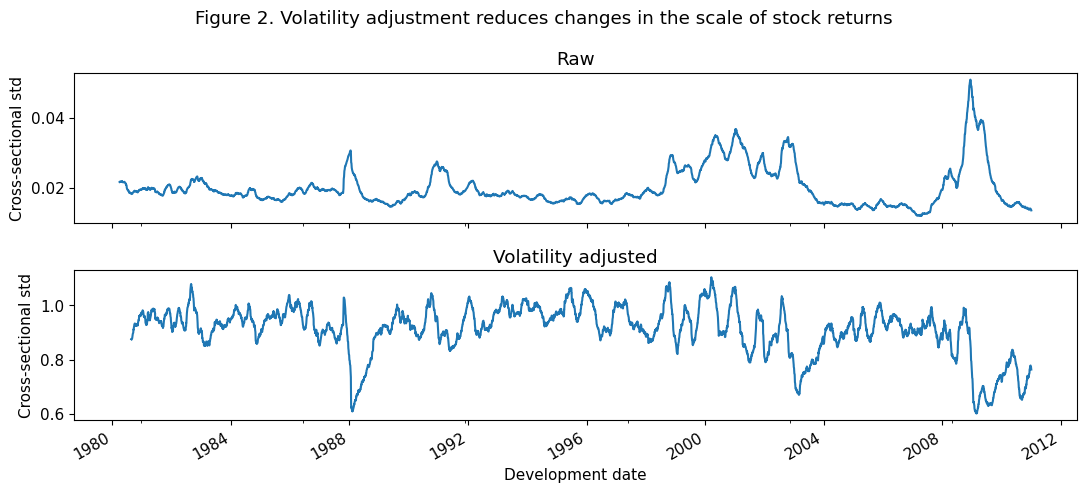
\includegraphics[width=\columnwidth]{../results/task3_compact/figures/figure-2.png}
\caption{Cross-sectional standard deviation of member returns (63-day average) before (top) and after (bottom) volatility adjustment.}
\label{fig:t3_voladj}
\end{figure}

\textit{Exploratory signal analysis.} Before fitting any model, we evaluated two classical effects as rule-based predictors. Short-term reversal, which predicts minus the mean adjusted return of the last five days, reaches a Sharpe ratio of 2.33 over 1985--2010 with a mean daily rank correlation of 0.026, but its Sharpe ratio falls from 4.09 in 1990--1994 to 1.25 in 2005--2010. Twelve-month momentum is much weaker, with a development Sharpe ratio of 0.52. These findings shape the method: past returns carry real but small predictive information, concentrated at short horizons; this information decays over time, so relationships must be re-estimated on recent data; and the heavy tails call for transformations that are robust to extreme values.

\subsection{Data Processing and Leakage Prevention}
\label{sec:t3_processing}

\textit{Target and features.} The training target is the next-day adjusted return, clipped to $[-5, 5]$ and demeaned across members each day. We built 18 return-based features from the clipped adjusted returns: 1-, 5- and 21-day reversal (the mean adjusted return over the last 1, 5 and 21 days), 12-1 month momentum (the sum over days $t-251$ to $t-21$, skipping the most recent month), the logarithm of $\hat\sigma_t$, sector-relative versions of the reversal and momentum features (net of the same-day mean of the stock's sector), and exponentially smoothed versions of these features with half-lives of 5 and 10 days. Six smoothed features whose correlation with their unsmoothed version exceeded 0.97 were dropped. Each feature is ranked across members each day and scaled to $[-0.5, 0.5]$, with missing values set to the neutral value 0, then standardized at each refit using the training rows only. Sentiment features (bullish, bearish, net and total scores, raw and smoothed, and an availability flag) are used from July 2009 onward.

\textit{Training and test sets.} We use a walk-forward procedure. At each refit date $d$, a model is trained on the member rows of the preceding three years, up to day $d-1$, and then predicts every day until the next refit, every 63 trading days for the Lasso and every 252 for the random forest and MLP. Non-member days are used only to estimate volatility and build features, never as training targets or for evaluation. The development period (1990--2010) is used for all model selection; the test period (2011--2013) was evaluated once, after the final configurations had been committed to our repository.

\textit{Leakage prevention.} Each feature on day $t$ uses only data up to day $t$, which a test verifies by recomputing all features from data truncated at 20 random dates and comparing them with the full-data values. The training code asserts that a model predicting on day $t$ is trained only on rows up to $t-1$, whose targets $\tilde r_t$ are known at the close of day $t$. Sentiment dated on calendar day $d$ is used only from the close of the first trading day after $d$, since posts may follow the market close. Two controls test the whole pipeline: shifting the features one day into the future raises the development Sharpe ratio of the Lasso from 4.06 to 68.3, while permuting the training targets within each day reduces it to $-0.02$, confirming that the pipeline detects leakage and that the models learn from real structure. Finally, the evaluation code was frozen before any model was trained.

\subsection{Proposed Solution}
\label{sec:t3_solution}

\textit{Models.} We compare three scikit-learn regressors~\cite{sklearn}. The Lasso~\cite{tibshirani1996} minimizes the squared error plus $\alpha\lVert\mathbf w\rVert_1$, which sets the weights of uninformative features to zero. The random forest~\cite{breiman2001} averages 100 regression trees, each grown on a random subsample of 200{,}000 training rows and considering one third of the features at each split. The MLP has one hidden layer of ReLU units and is trained on the squared error with an L2 weight penalty. The baselines are the 5-day reversal and 12-1 momentum rules of Section~\ref{sec:t3_analysis}, applied without fitting.

\textit{Hyperparameter tuning.} For the Lasso, we searched six penalties $\alpha$ from $1.7\times10^{-4}$ to $1.7\times10^{-2}$ with three-year, five-year and expanding training windows. For the random forest, we searched maximum depths $\{4, 6, 8\}$ and minimum leaf sizes $\{200, 1000\}$, and for the MLP, 16 or 32 hidden units and L2 penalties $\{10^{-4}, 10^{-2}\}$, with the number of epochs chosen on the most recent 20\% of each training window. Configurations were ranked by development Sharpe ratio, preferring consistency across the four windows 1990--1994, 1995--1999, 2000--2004 and 2005--2010 over a higher total driven by one window. The best configuration of every family lay at the edge of its grid, so we extended each grid by one step, fixing in advance that a configuration would only be replaced if the extension improved its development Sharpe ratio by more than one standard error (0.22). The final configurations are a Lasso with $\alpha = 1.7\times10^{-4}$ refit every 63 days, a random forest of depth 12 with leaves of at least 200 rows, and an MLP with 32 hidden units, penalty $10^{-4}$ and up to 60 epochs, the latter two refit every 252 days, all on three-year windows.

\textit{Prediction smoothing.} To lengthen the holding period, each stock's predictions can be replaced by an exponentially weighted average of its past predictions, with weights that halve every $h$ days. As a fourth finalist, we smooth the MLP's predictions with $h = 5$, a choice fixed before its development performance was computed.

\textit{Implementation.} The group inspected and cleaned the data, implemented the volatility adjustment and the evaluation code, and validated them. An LLM agent, Claude Code~\cite{claudecode}, then implemented the features and ran the experiments under a written protocol, reproduced in the appendix of the submitted notebook; Section~\ref{sec:t3_rationale} explains how this protocol limits overfitting, and Section~\ref{sec:llm} describes our LLM usage.

\subsection{Design Rationale}
\label{sec:t3_rationale}

\textit{Low signal and high noise.} The mean daily rank correlation of the reversal rule is only 0.026, so most of the variation in returns is noise. Volatility adjustment gives every stock and period a comparable scale. Ranking the features and clipping the targets limit the influence of the heavy tails, which would otherwise dominate a squared-error fit. Demeaning the target removes the market's common move, which no stock-level feature can predict, and focuses the models on returns relative to one another. Model capacity is kept small: the random forest uses large leaves and subsampled rows, the MLP has at most 32 hidden units and an L2 penalty, and the Lasso's L1 penalty removes features that do not help. A small, fixed set of features built from well-documented effects also limits the number of spurious relationships the models can find.

\textit{Non-stationarity.} Section~\ref{sec:t3_analysis} showed that predictability decays over time. We therefore re-estimate each model regularly on a trailing three-year window, which outperformed an expanding window for the Lasso (development Sharpe ratio 4.06 against 3.09), and select configurations that perform consistently across sub-periods rather than in a single favourable one.

\textit{Overfitting through repeated testing.} Comparing many configurations on the same data inflates the best result even without leakage. We restricted the search to small grids declared before the experiments, recorded every configuration tried (62 before the final selection, of which 55 were eligible and 7 were controls or diagnostics), fixed the one-standard-error replacement rule before extending the grids, and evaluated each finalist on the test period exactly once. Before that evaluation, we recorded an expected range for each test Sharpe ratio, so the test result could be judged against a prior expectation. Delegating the experiments to an agent made these rules essential: the agent could not modify the evaluation code (checked against the frozen version at every review), could not commit to the repository, stopped for human review after each of its five phases, and logged every decision. It also disclosed three minor deviations from the test lockout, none affecting a fitted model: it printed counts, but not values, of test-period returns while mapping sentiment onto duplicated identifiers, after which we required that mapping to use data up to 2010 only; the last development prediction, on December 31, 2010, is scored on the first test-period return; and we had evaluated the reversal rule through 2013 while validating the evaluation code.

\textit{Holding period and sentiment.} Short holding periods mean high trading costs, so we tested smoothing half-lives of 2, 5 and 10 days to measure the trade-off with the Sharpe ratio. Because sentiment is available for only 18 months before the test period, sentiment models were developed on 2010 alone, with at most six configurations, to avoid fitting noise.

\subsection{Evaluation Metrics}
\label{sec:t3_metrics}

\textit{Sharpe ratio.} Following the assignment, the portfolio invests in each stock in proportion to its predicted return divided by its estimated volatility, so its daily profit-and-loss (P\&L) is
\begin{equation}
R_t = \sum_i \hat r_{t,i}\,\tilde r_{t+1,i},
\end{equation}
where the sum is over members on day $t$ and $\hat r_{t,i}$ is the prediction, demeaned across stocks each day. We use unclipped returns, which are what a strategy would actually earn. The annualized Sharpe ratio is $\mathrm{SR} = \sqrt{252}\,\overline{R}/\mathrm{sd}(R)$, with no benchmark subtracted and 252 trading days per year. It measures return per unit of risk, which mean squared error does not capture. Under a Gaussian assumption, its standard error is roughly $1/\sqrt{\tau}$ for $\tau$ years of data: about 0.58 on the three-year test period and 0.22 on the 21-year development period. We report it over the full period, by window and by year, because a strategy that works only in the 1990s is not useful today, and we plot the cumulative P\&L to show whether performance is steady.

\textit{Rank correlation.} The information coefficient (IC) is the daily Spearman correlation between predicted and realized returns across stocks. Unlike the Pearson correlation, it measures whether the predicted ordering is correct and is robust to extreme returns. We report its mean, its $t$-statistic (the mean divided by its standard deviation, times the square root of the number of days) and its cumulative sum over time.

\textit{Holding period and market exposure.} The average holding period $H_{av}$ is computed with the assignment's formula, averaging over stocks with at least 20 predictions; it approximates how long a position is held and therefore how costly the strategy is to trade. Finally, we report the Pearson correlation $\rho_{\mathrm{mkt}}$ of $R_t$ with an equal-weight long-only portfolio of members, since returns have a positive mean and any predictor biased towards buying looks profitable. The assignment suggests that a Sharpe ratio of about 2 is needed for one-day holding periods and 0.8 to 1 for 3 to 5 days.

\textit{Validation of the evaluation code.} Before any model was trained, perfect-foresight predictions gave a Sharpe ratio of 16.6 on the test period, confirming that predictions and returns are correctly aligned; random predictions gave 0.31, within the noise expected over three years; and an always-long portfolio gave a market correlation of 1.00.

\subsection{Results}
\label{sec:t3_results}

\textit{Development period.} Table~\ref{tab:t3_dev} reports the development results of the baselines and of each finalist. All fitted models beat the reversal rule, and the ordering of random forest and MLP above Lasso above reversal holds in every window. Performance decays steadily: every model loses about three quarters of its Sharpe ratio between 1990--1994 and 2005--2010, which makes the last window the best guide to test performance. Part of the early predictability likely reflects bid-ask bounce, since prices were quoted in fractions of a dollar before 2001. Differences within a family are small relative to the standard error of 0.22. In the grid extension, ordinary least squares improved on the Lasso by only 0.14, confirming a plateau, whereas deeper trees and longer MLP training cleared the replacement threshold narrowly (by 0.28 and 0.24).

\begin{table}[t]
\caption{Development-period results (walk-forward predictions, 1990--2010). SR: annualized Sharpe ratio, overall and by window; $H_{av}$: average holding period in days. Smoothed MLP: MLP predictions smoothed with a half-life of 5 days.}
\label{tab:t3_dev}
\centering
\footnotesize
\setlength{\tabcolsep}{3pt}
\begin{tabular}{lcccccc}
\toprule
Model & SR & 90--94 & 95--99 & 00--04 & 05--10 & $H_{av}$ \\
\midrule
5-day reversal & 2.18 & 4.09  & 2.59 & 1.39    & 1.25 & 1.56 \\
12-1 momentum  & 0.52 & 0.85  & 1.22 & $-0.01$ & 0.23 & 10.91 \\
Lasso          & 4.06 & 7.48  & 4.77 & 2.60    & 1.81 & 1.39 \\
Random forest  & 5.78 & 10.19 & 6.49 & 4.14    & 2.70 & 1.09 \\
MLP            & 5.39 & 9.20  & 6.33 & 3.86    & 2.69 & 1.27 \\
Smoothed MLP   & 2.53 & 4.02  & 3.46 & 1.71    & 1.43 & 5.56 \\
\bottomrule
\end{tabular}
\end{table}

\textit{Smoothing and sentiment.} Smoothing trades Sharpe ratio for holding period (Table~\ref{tab:t3_smooth}). For the MLP, a half-life of 5 days lengthens the holding period from 1.3 to 5.7 days and reduces the development Sharpe ratio from 5.16 to 2.45, still well above the benchmark for that horizon. Sentiment did not help: in 2010, adding sentiment features to the Lasso gave Sharpe ratios of 0.32 to 0.37, against 0.37 to 0.43 without, a sentiment-only Lasso scored $-0.90$, and a random forest with sentiment (1.32) did worse than the random forest on return features alone (3.67). With a standard error of about 1.0 for one year, none of these differences is significant, and no sentiment model was retained.

\begin{table}[t]
\caption{Effect of smoothing the predictions with half-life $h$ days (initial-grid configurations): development Sharpe ratio / average holding period in days.}
\label{tab:t3_smooth}
\centering
\small
\begin{tabular}{lccc}
\toprule
$h$ & Lasso & Random forest & MLP \\
\midrule
0  & 4.06 / 1.39 & 5.50 / 1.14 & 5.16 / 1.29 \\
2  & 2.86 / 3.55 & 3.79 / 2.95 & 3.55 / 3.30 \\
5  & 2.08 / 6.27 & 2.53 / 5.23 & 2.45 / 5.73 \\
10 & 1.61 / 9.92 & 1.76 / 8.29 & 1.75 / 8.87 \\
\bottomrule
\end{tabular}
\end{table}

\textit{Test period.} Table~\ref{tab:t3_test} and Fig.~\ref{fig:t3_test} report the single evaluation on 2011--2013. The expected range of each Sharpe ratio, recorded beforehand, runs from one more step of the decay observed between development windows to no further decay, widened by one standard error on each side. All four finalists beat both baselines. The random forest (3.65) and the MLP (3.01) were profitable in each test year, their cumulative rank correlation rises throughout the period, and their IC $t$-statistics exceed 5, so their rankings of stocks carry information. The two metrics do not always agree: 12-1 momentum has a mean rank correlation similar to theirs (0.019) but a Sharpe ratio of only 0.79, because its daily rank correlation is much more variable, as its lower IC $t$-statistic shows. Both held or exceeded their 2005--2010 level, whereas the Lasso (1.81 to 1.07) and the reversal rule (1.25 to 0.73) continued to decay. The Lasso's margin over the reversal rule is only about 0.6 standard errors, and the gap between the random forest and the MLP, about one standard error, does not establish that either is better. The random forest exceeded the upper end of its expected range. Before accepting this result, we verified that the walk-forward reproduced all development results exactly, that every training window ended before its refit date, and that recomputing features, targets and predictions after deleting all data beyond June 2012 left every earlier prediction unchanged. A plausible explanation, found only after seeing the result, is that the 2005--2010 reference is depressed by 2008: the forest's mean yearly Sharpe ratio over 2005--2010 is 3.02. The smoothed MLP reached 1.40 with a holding period of 4.5 days, but almost all of it came in 2012 and 2013 (2011: 0.11), and its IC $t$-statistic of 1.84 is weak.

\begin{table}[t]
\caption{Test-period results (2011--2013), each finalist evaluated once. Expected: Sharpe ratio range recorded before the evaluation; IC $t$: $t$-statistic of the mean daily rank correlation; $\rho_{\mathrm{mkt}}$: correlation with the equal-weight market.}
\label{tab:t3_test}
\centering
\small
\setlength{\tabcolsep}{3.5pt}
\begin{tabular}{lccccc}
\toprule
Model & Expected & SR & IC $t$ & $H_{av}$ & $\rho_{\mathrm{mkt}}$ \\
\midrule
5-day reversal & 0.2--1.8     & 0.73 & 1.87 & 1.61  & 0.15 \\
12-1 momentum  & $-0.4$--0.8  & 0.79 & 3.21 & 11.44 & 0.12 \\
Lasso          & 0.6--2.4     & 1.07 & 2.67 & 1.48  & 0.38 \\
Random forest  & 1.2--3.3     & 3.65 & 5.55 & 0.94  & 0.39 \\
MLP            & 1.2--3.3     & 3.01 & 5.65 & 1.04  & 0.31 \\
Smoothed MLP   & 0.35--2.0    & 1.40 & 1.84 & 4.51  & 0.40 \\
\bottomrule
\end{tabular}
\end{table}

\begin{figure}[t]
\centering
%\safefig{fig_t3_test.pdf}
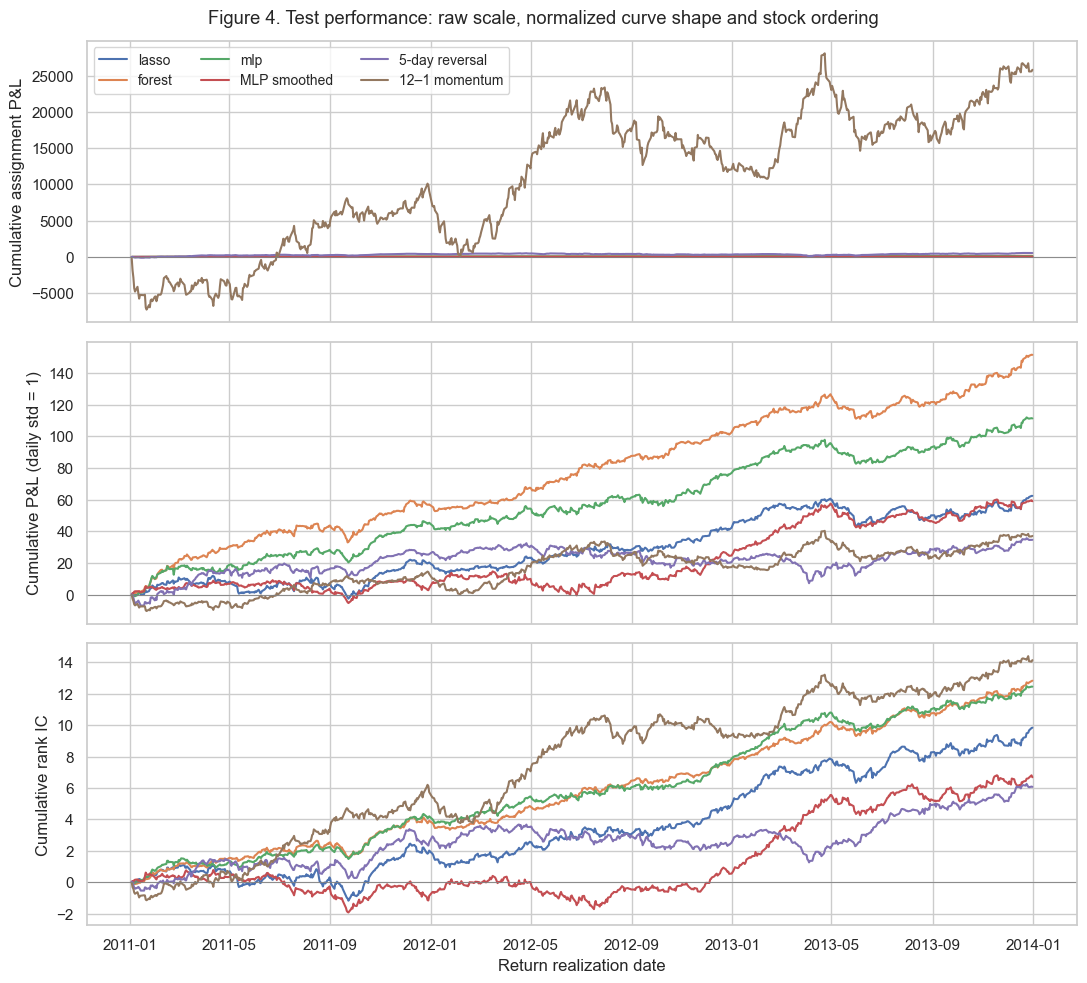
\includegraphics[width=\columnwidth]{../results/task3_compact/figures/figure-4.png}
\caption{Test period (2011--2013): cumulative P\&L, each series divided by its own daily standard deviation so slopes are comparable (top), and cumulative daily rank correlation (bottom), for the finalists and baselines.}
\label{fig:t3_test}
\end{figure}

\textit{Execution timing and market exposure.} All Sharpe ratios exclude transaction costs and assume that trades execute at the closing prices used to form the predictions. To measure this dependence, we re-scored each finalist with its predictions applied one day late (Table~\ref{tab:t3_robust}); the test-period diagnostics are post-hoc analyses of the frozen predictions. In development, the fitted models kept about two thirds of their Sharpe ratio, while the reversal rule kept all of it. On the test period, the random forest and MLP kept only about one third (1.24 and 1.02), which leaves the random forest only 0.55, about one standard error, above the reversal rule; the Lasso and the smoothed MLP kept about two thirds. Daily demeaning also does not make the strategies market neutral: each finalist's P\&L has a test correlation of 0.31 to 0.40 with the equal-weight market, whose own Sharpe ratio over the period was 1.10. Subtracting the fitted market exposure barely changes the random forest and MLP (3.50 and 2.81), whereas the Lasso falls from 1.07 to 0.70, so much of its test performance was market exposure.

\begin{table}[t]
\caption{Robustness: Sharpe ratio with on-time and one-day-late execution in development and test, and test Sharpe ratio after subtracting the fitted market exposure (hedged).}
\label{tab:t3_robust}
\centering
\footnotesize
\setlength{\tabcolsep}{3pt}
\begin{tabular}{lccccc}
\toprule
 & \multicolumn{2}{c}{Development} & \multicolumn{3}{c}{Test} \\
\cmidrule(lr){2-3}\cmidrule(lr){4-6}
Model & On time & Late & On time & Late & Hedged \\
\midrule
5-day reversal & 2.18 & 2.29 & 0.73 & 0.69 & 0.56 \\
Lasso          & 4.06 & 2.70 & 1.07 & 0.72 & 0.70 \\
Random forest  & 5.78 & 3.81 & 3.65 & 1.24 & 3.50 \\
MLP            & 5.39 & 3.55 & 3.01 & 1.02 & 2.81 \\
Smoothed MLP   & 2.53 & --   & 1.40 & 0.93 & 1.04 \\
\bottomrule
\end{tabular}
\end{table}

\subsection{Conclusion}
\label{sec:t3_conclusion}

Past returns contain genuine short-horizon information about relative stock returns. The random forest and MLP captured it on the test period, about five to six standard errors from zero, and hedging their market exposure barely changed them; their mean daily rank correlation is only 0.018, but with about 500 predictions per day this small edge accumulates. The Lasso's coefficients shrank steadily over time (the sum of their absolute values averaged 0.24 in 1990--1994, 0.18 in 2005--2010 and 0.08 during the test period), and sentiment added nothing measurable. However, most of the nonlinear models' advantage requires trading at the close used to form the prediction; applied one day late, they come within about one standard error of the reversal rule. The smoothed MLP, which keeps two thirds of its Sharpe ratio when delayed (0.93 at a holding period of 4.5 days), is therefore the most credible result. Future work should train on an execution-lagged target (the return from $t+1$ to $t+2$), include transaction costs in model selection, build market- and sector-neutral portfolios, control the false discovery rate across features, and revisit sentiment with a longer history.


% ==================================================================
\section{Discussion and Conclusion}
\label{sec:conclusion}
% ==================================================================
% Grid: summarizes findings (1) and suggests improvements (1).
The first regression task included a statistical analysis, determining that scaling would be beneficial for model implementation. For the classification task, the classification models were evaluated by comparing their prediction accuracy with Scikit-learn implementation, demonstrating similar results (94.83\% and 96.66\% vs. 95.63\%). The hyperparameter studies demonstrate why selecting appropriate model parameters is important, as balancing regularization strength, model capacity, and learning rate prevents underfitting, overfitting, and gradient overshooting. Improvements could be made in the optimization algorithm, such as using mini batch gradient descent or Adam to improve computational efficiency and convergence, incorporating early-stopping, or using non-linear kernel SVM. Across the assignment, proper data preprocessing, regularization, and disciplined hyperparameter tuning consistently proved more critical to generalization than model complexity alone. In Task 3, the main lesson is that, with financial data, how a model is evaluated matters as much as which model is used: careful protocols against lookahead and repeated testing, and diagnostics such as delayed execution, changed how strong our results appeared.


% ==================================================================
\section{Statement of Contributions}
% ==================================================================
This assignment was broken down as follows: Jocelyn Poon worked on the regression portion of task 1 and 2, Ruiyong Xu worked on the classification portion of task 1 and 2, finally Louis Salanon and Maxime Robatche-Claive focused on task 3. All members were assigned to write their own report section based on their task, and everyone reviewed the full submission.


% ==================================================================
\section{Statement on LLM Usage}
\label{sec:llm}
% ==================================================================
Chat GPT was used in the regression task to help generate plots and verify the implementation of the models. Our implementation of the MLP class referenced the code output by ChatGPT, prompted by passing the given MLP Python class template and asking it to give a minimal implementation. For Task 3, we used Claude (Anthropic, model Claude Opus 5.5, chat interface) interactively to plan the division of work, to guide the inspection and cleaning of the data, and to suggest code for volatility adjustment and evaluation, which we ran, checked against controls and modified ourselves. The same assistant drafted the agent prompt and an initial version of the Task 3 text in this report, both of which we reviewed and edited. Experiments were then run with Claude Code (Opus 5.5 High from \texttt{/model} in Claude Code) inside our repository. Its context consisted of the repository, our exploration notebook and the written prompt, reproduced in the appendix of the submitted notebook together with a summary of the agent's log, which records its decisions and the questions it asked us. We reviewed the agent's output at each of its five checkpoints, made all commits ourselves, and approved the finalists before the test evaluation.


% ==================================================================
\begin{thebibliography}{9}
\bibitem{sklearn} F. Pedregosa \emph{et al.}, ``Scikit-learn: Machine learning in Python,'' \emph{J. Mach. Learn. Res.}, vol. 12, pp. 2825--2830, 2011.
\bibitem{tibshirani1996} R. Tibshirani, ``Regression shrinkage and selection via the lasso,'' \emph{J. Roy. Stat. Soc. B}, vol. 58, no. 1, pp. 267--288, 1996.
%\bibitem{zou2005} H. Zou and T. Hastie, ``Regularization and variable selection via the elastic net,'' \emph{J. Roy. Stat. Soc. B}, vol. 67, no. 2, pp. 301--320, 2005.
%\bibitem{cortes1995} C. Cortes and V. Vapnik, ``Support-vector networks,'' \emph{Mach. Learn.}, vol. 20, no. 3, pp. 273--297, 1995.
%\bibitem{breiman2001} L. Breiman, ``Random forests,'' \emph{Mach. Learn.}, vol. 45, no. 1, pp. 5--32, 2001.
\bibitem{claudecode} Anthropic, ``Claude Code,'' 2026. [Online]. Available: \url{https://docs.claude.com}
\end{thebibliography}

\end{document}
